\section{Results}
\label{sec:results}
All results use real hospitals as released: the 19 PCa-19 hospitals and, in Section~\ref{sec:heart}, the four heart-disease hospitals. We first summarise the federation that is valued (Section~\ref{sec:federation}); its full analysis is in Supplementary Section~\ref{S-sec:pca19_more}. We then turn to valuation under DP (Sections~\ref{sec:p19_retrain}--\ref{sec:heart}).

\subsection{The Federation Being Valued}
\label{sec:federation}
Our re-implementation of the base paper's protocol reproduces the authors' released code to within $1.2\times10^{-14}$ for both of their calculators (Supplementary Section~\ref{S-sec:p19_repro}), and its sustainability finding holds under our protocol: joining brings no significant average gain over local training (FL$-$LOC $=\pDFLminusLOC$), a free-rider obtains almost the same model (FR$-$FL $=\pDFRminusFL$), and federated training matches pooled training (CEN$-$FL $=\pDCENminusFL$). For this seven-parameter, regularised logistic calculator trained on \pNineN{} patients, DP changes the mean per-hospital AUC by only $\pDpLossHalf$ even at $\varepsilon=0.5$. We do not generalise this: the cost of a given $\varepsilon$ depends strongly on the model and the amount of data, and for a federated MLP the same budgets perturb the released models far more (Section~\ref{sec:p19_mlp}). Discrimination transports to held-out countries, but calibration does not (observed/expected ratios \pOeMin--\pOeMax); an intercept update on 20\% of a new country's patients, which is common clinical practice for risk calculators anyway, reduces $|\log\mathrm{O/E}|$ from \pRecalOeRaw{} to \pRecalOeInt{} (Supplementary Section~\ref{S-sec:p19_loco}).

\subsection{Retraining-Based Valuation under DP}
\label{sec:p19_retrain}
Following standard practice, we first retrain every coalition with DP at a per-run $\varepsilon$ and compute exact Shapley values over the ten largest hospitals (1{,}023 coalitions). Their agreement with the non-private ranking falls from Spearman $\rho=\pShRhoTen$ at $\varepsilon=10$ to \pShRhoTwo{} at $\varepsilon=2$ and \pShRhoHalf{} at $\varepsilon=0.5$ (original splits, against the no-DP ranking; Table~\ref{S-tab:osa} repeats this on the held-out splits against exact Shapley), although the federation's AUC changes by less than 0.01 over this range. Leave-one-out values are near zero for every hospital and cannot separate contributors (Spearman with Shapley \pShLooRho). These results ignore the cost of the valuation itself.

\subsection{Valuation at an Honest Privacy Budget}
\label{sec:p19_osa}
Table~\ref{S-tab:osa} makes the real cost of retraining explicit: with ten hospitals each hospital joins 512 private training runs, so a per-run $\varepsilon$ of 10, 5 or 1 corresponds to a total $\varepsilon$ of about \trueEpsTen{}, \trueEpsFive{} and \trueEpsOne{} per hospital. When the total budget is held at the stated $\varepsilon$ (\emph{budget-matched} retraining), every run needs much more noise and the ranking is lost: Spearman $\rho$ with the exact non-private Shapley values falls to \bmRhoTen{} at $\varepsilon=10$ and \bmRhoOne{} at $\varepsilon=1$.

OSA-Shapley (Section~\ref{sec:osa}) spends the budget once. Without DP it reproduces the retraining Shapley ranking almost exactly ($\rho=\osaNoDP$), and under DP it keeps $\rho=\osaRhoTen$ at $\varepsilon=10$, \osaRhoTwo{} at $\varepsilon=2$, \osaRhoOne{} at $\varepsilon=1$ and \osaRhoHalf{} at $\varepsilon=0.5$ (Table~\ref{S-tab:osa}; evaluated on 20 splits that were not used to choose its single hyper-parameter). At equal privacy it beats retraining by $\osaVsBmTwo$ in $\rho$ at $\varepsilon=2$. At $\varepsilon=2$ it matches per-run retraining ($\osaVsPrTwo$), which spends 28--42 times more privacy. Because no coalition needs training, exact valuation of all 19 hospitals is feasible: the OSA ranking computed with DP agrees with the non-private one at $\rho=\osaNineRhoFive$ ($\varepsilon=5$) and \osaNineRhoOne{} ($\varepsilon=1$).


\subsection{Against Valuations that Also Cost the Budget Once}
\label{sec:p19_post}
The fair competitors are the reconstruction methods MR and OR, which post-process the DP-FedAvg run (Section~\ref{sec:osa}). Table~\ref{S-tab:osa_post} and Fig.~\ref{S-fig:osa} compare them on the same splits. For the ten largest hospitals, OSA-Shapley is more accurate than exact MR, the upper bound for GTG-Shapley, at every privacy level: $\rho$ \osaRhoTwo{} vs \mrRhoTwo{} at $\varepsilon=2$ (difference \osaVsMrTwo) and \osaRhoOne{} vs \mrRhoOne{} at $\varepsilon=1$ (\osaVsMrOne). It also beats OR by \osaVsOrTwo{} at $\varepsilon=2$. The gap is already present without DP ($\rho$ \osaNoDP{} vs \mrRhoNoDP), so it comes from the coalition proxy rather than from the noise.


\subsection{Is OSA-Shapley Worth It? Cheap Proxies}
\label{sec:p19_proxies}
A federation could avoid a valuation protocol altogether and credit hospitals by what they can share cheaply. Table~\ref{tab:proxies} compares these proxies with OSA-Shapley against the same exact non-private reference. For the ten largest hospitals, hospital size, the number of cancer cases and the similarity of summary statistics to the pooled ones carry almost no information about contribution ($\rho$ \pxLSizeNoDP, \pxLPosNoDP{} and \pxLStatNoDP; OSA$-$size $=\pxdLSizeTwo$ at $\varepsilon=2$). They also cannot detect a hospital with useless data, because random labels change neither its size nor its prevalence (0\% of splits). Hospitals here differ in case mix, not only in size, and their marginal value depends on what the other hospitals already provide. An AUC that each hospital reports for its own model is unverifiable and agrees poorly with the ranking ($\rho=\pxLOwnTwo$ at $\varepsilon=2$).

Proxies built on a released model behave differently. Once each hospital has released one DP model, as OSA requires, the AUC of that single model on the reference set already ranks the large hospitals well ($\rho=\pxLRefTwo$ at $\varepsilon=2$) and flags the useless hospital. OSA-Shapley is comparable at $\varepsilon=2$ ($\pxdLRefTwo$) and better at $\varepsilon=1$ ($\pxdLRefOne$), where single releases are noisy and averaging over coalitions helps; it also beats the leave-one-out value of the averaged releases by $\pxdLLooTwo$. Both scores use the same releases, so OSA's advantage costs no extra privacy or communication. OSA's values are also Shapley values: they sum to the federation's gain over chance, which a single-model score does not.

On the ten smallest hospitals the picture changes (Table~\ref{tab:proxies}, right). There contribution is driven mainly by data volume, and hospital size alone reaches $\rho=\pxSSizeNoDP$. At $\varepsilon=2$, OSA-Shapley, MR, the single-model score and size agree with the ranking about equally well (OSA$-$size $=\pxdSSizeTwo$, OSA$-$MR $=\pxdSMrTwo$), and at $\varepsilon=1$ none of the DP valuations is better than size.

\begin{table*}[t]
\caption{Is OSA-Shapley worth its cost? Agreement (Spearman $\rho$) of cheap contribution proxies and of privacy-honest valuations with the exact non-private retraining Shapley ranking, on real PCa-19 hospitals (20 held-out splits). \emph{What is shared}: what each hospital must reveal. Proxies that use a model use the same DP releases as OSA-Shapley and therefore cost the same $\varepsilon$; size, counts and statistics are shared without DP. \emph{Useless}: share of splits in which a hospital whose training labels were replaced by random labels (es6) is ranked last at $\varepsilon=2$; a tie for last place does not count.}
\centering\scriptsize
\setlength{\tabcolsep}{4pt}
\begin{tabular}{llccccccc}
\toprule
 & & \multicolumn{4}{c}{Ten largest hospitals} & \multicolumn{3}{c}{Ten smallest hospitals} \\
\cmidrule(lr){3-6}\cmidrule(lr){7-9}
Contribution score & What is shared & no DP & $\varepsilon=2$ & $\varepsilon=1$ & Useless & no DP & $\varepsilon=2$ & $\varepsilon=1$ \\
\midrule
Hospital size $n_k$ & size (public) & 0.08 & 0.08 & 0.08 & 0\% & 0.74 & 0.74 & 0.74 \\
Number of csPCa cases & one count & 0.02 & 0.02 & 0.02 & 0\% & 0.50 & 0.50 & 0.50 \\
Similarity of summary statistics & feature means, prevalence & \ensuremath{-}0.18 & \ensuremath{-}0.18 & \ensuremath{-}0.18 & 0\% & 0.72 & 0.72 & 0.72 \\
Self-reported local AUC & one AUC (unverifiable) & 0.36 & 0.25 & 0.26 & 100\% & 0.40 & 0.54 & 0.56 \\
Single-model AUC on reference set & one DP model ($\varepsilon$) & 0.93 & 0.85 & 0.71 & 100\% & 0.94 & 0.79 & 0.72 \\
Leave-one-out of averaged models & one DP model ($\varepsilon$) & 0.85 & 0.77 & 0.74 & 0\% & 0.59 & 0.34 & 0.34 \\
OR reconstruction & DP-FedAvg run ($\varepsilon$) & 0.42 & 0.51 & 0.50 & 100\% & 0.79 & 0.74 & 0.59 \\
MR reconstruction (GTG bound) & DP-FedAvg run ($\varepsilon$) & 0.74 & 0.75 & 0.65 & 70\% & 0.86 & 0.78 & 0.74 \\
Retraining, budget-matched & $2^{K-1}$ runs ($\varepsilon$) & -- & 0.18 & 0.10 & 60\% & -- & 0.45 & 0.29 \\
\textbf{OSA-Shapley (ours)} & one DP model ($\varepsilon$) & \textbf{0.96} & \textbf{0.89} & \textbf{0.80} & 100\% & \textbf{0.95} & \textbf{0.79} & \textbf{0.68} \\
\bottomrule
\end{tabular}
\label{tab:proxies}
\end{table*}


\subsection{A Hospital with Useless Data, Removal and Robustness}
\label{sec:p19_robust}
We replaced the training labels of one mid-sized hospital (\corrHosp) by random labels and asked whether each valuation ranks it last (Tables~\ref{tab:proxies} and~\ref{S-tab:osa_robust}). The non-private retraining Shapley values always do (\corrTruth). At $\varepsilon=2$ and $\varepsilon=1$, OSA-Shapley ranks it last in \corrOsaTwo{} and \corrOsaOne{} of splits, MR in \corrMrTwo{} and \corrMrOne, and budget-matched retraining in only \corrBmTwo{} and \corrBmOne; no size- or statistics-based proxy ever does. Sensitivity to the reference-set size and the number of local steps is reported in Table~\ref{S-tab:osa_robust}.

\subsection{A Non-Convex Model}
\label{sec:p19_mlp}
OSA-Shapley assumes that averaging locally trained models approximates the federated model of a coalition, which holds for convex losses. We therefore repeated the comparison with a one-hidden-layer MLP (16 tanh units) trained by FedAvg, with exact non-private retraining Shapley values of the federated MLP as the reference (Table~\ref{S-tab:osa_mlp}). Because averaging the parameters of separately trained networks is fragile, the coalition prediction is the size-weighted average of the members' log-odds (OSA-ens.), which is equally post-processing. Without DP the ensemble variant reproduces the reference ranking well ($\rho=\mlpOsaNoDP$, against \mlpMrNoDP{} for MR). Under DP it loses this advantage: at $\varepsilon=2$ and $\varepsilon=1$ it reaches \mlpOsaTwo{} and \mlpOsaOne{}, whereas MR reaches \mlpMrTwo{} and \mlpMrOne{} (OSA$-$MR $=\mlpOsaVsMrTwo$ at $\varepsilon=2$). A non-linear model trained alone for 200 noisy steps accumulates the DP perturbation, whereas MR's short local updates restart from the shared global model in every round. Budget-matched retraining of the MLP is close to chance ($\rho=\mlpBmTwo$; \mlpBmSeeds{} splits). For non-convex models, reconstruction from the training run is the better privacy-honest valuation.


\subsection{Small Hospitals: Where OSA-Shapley Loses Its Advantage}
\label{sec:p19_small}
To study small silos without simulating any, we value the ten smallest PCa-19 hospitals (\pxSmallMin--\pxSmallMax{} patients; exact non-private retraining Shapley as reference, 20 held-out splits). Without DP, OSA-Shapley is again the most accurate valuation ($\rho=\pxSOsaNoDP$; OSA$-$MR $=\pxdSMrNoDP$). Under DP its advantage disappears: at $\varepsilon=2$ OSA and MR agree with the ranking equally well (\pxSOsaTwo{} and \pxSMrTwo{}; difference $\pxdSMrTwo$), and at $\varepsilon=1$ MR is slightly, not significantly, ahead (\pxdSMrOne). Budget-matched retraining remains far worse ($\rho=\pxSBmTwo$ at $\varepsilon=2$). This is the regime that Proposition~3 predicts: the release of a hospital with a few dozen patients carries noise of order $\sigma/n_k$, whereas reconstruction averages over the federation in every round. With hospitals this small, hospital size is itself a strong proxy (Section~\ref{sec:p19_proxies}), and no privacy-honest valuation improves on it at $\varepsilon \le 1$.


\subsection{A Second Real Federation: Heart Disease}
\label{sec:heart}
Table~\ref{tab:heart} repeats the comparison on the four hospitals of the UCI Heart Disease collection, with OSA-Shapley's PCa-19 hyper-parameters unchanged. Without DP the picture is the same as before: OSA-Shapley recovers the exact ranking best ($\rho=\hrOsaNoDP$, against \hrMrNoDP{} for MR and \hrRefNoDP{} for the single-model score; OSA$-$MR $=\hrdMrNoDP$). Under DP it is not. These hospitals have 98--242 training patients for 21 model parameters, and their contributions are nearly equal (Shapley values \hrPhiMin--\hrPhiMax{} AUC), so the noise of a single release dominates. At $\varepsilon=5$ OSA-Shapley and MR are close (\hrOsaFive{} and \hrMrFive{}); at $\varepsilon=2$ MR is better (\hrMrTwo{} vs \hrOsaTwo{}; OSA$-$MR $=\hrdMrTwo$); and at $\varepsilon=1$ no valuation agrees with the ranking beyond chance. Retraining does not help: with four hospitals its composed cost is modest (a stated $\varepsilon=2$ really costs \hrTrueTwo), yet per-run and budget-matched retraining reach only \hrPrTwo{} and \hrBmTwo{}. Hospital size is anti-correlated with contribution ($\rho=\hrSizeNoDP$): the smallest hospital, Zurich/Basel, contributes most. Released models still detect bad data: OSA-Shapley and the single-model score rank \hrCorrupt{} with random labels last in \hrCOsaTwo{} and \hrCRefTwo{} of splits at $\varepsilon=2$, hospital size in \hrCSizeTwo.

\begin{table}[t]
\caption{Second real federation: the four hospitals of the UCI Heart Disease collection (Cleveland (303), Budapest (294), Zurich/Basel (123), Long Beach VA (200) patients), coronary artery disease, 20 held-out splits. Spearman $\rho$ with the exact non-private retraining Shapley ranking; with four hospitals $\rho$ moves in steps of 0.2. Per-run retraining really costs $\varepsilon\approx16$, 6.1 and 2.9 at a stated 5, 2 and 1. \emph{Useless}: share of splits in which Budapest, given random training labels, is ranked last at $\varepsilon=2$.}
\centering\scriptsize
\setlength{\tabcolsep}{3pt}
\begin{tabular}{lccccc}
\toprule
Contribution score & no DP & $\varepsilon=5$ & $\varepsilon=2$ & $\varepsilon=1$ & Useless \\
\midrule
Hospital size $n_k$ & \ensuremath{-}0.38 & \ensuremath{-}0.38 & \ensuremath{-}0.38 & \ensuremath{-}0.38 & 0\% \\
Similarity of summary statistics & \ensuremath{-}0.38 & \ensuremath{-}0.38 & \ensuremath{-}0.38 & \ensuremath{-}0.38 & 0\% \\
Self-reported local AUC & \ensuremath{-}0.18 & \ensuremath{-}0.17 & \ensuremath{-}0.31 & \ensuremath{-}0.30 & 70\% \\
Single-model AUC on reference set & 0.76 & 0.42 & \ensuremath{-}0.04 & \ensuremath{-}0.34 & 100\% \\
Leave-one-out of averaged models & 0.82 & 0.69 & 0.42 & 0.18 & 85\% \\
OR reconstruction & 0.23 & 0.29 & 0.18 & 0.04 & -- \\
MR reconstruction (GTG bound) & 0.70 & 0.64 & 0.45 & \ensuremath{-}0.35 & -- \\
Retraining, per run & -- & 0.34 & \ensuremath{-}0.09 & \ensuremath{-}0.27 & -- \\
Retraining, budget-matched & -- & \ensuremath{-}0.02 & \ensuremath{-}0.18 & \ensuremath{-}0.15 & -- \\
\textbf{OSA-Shapley (ours)} & \textbf{0.92} & \textbf{0.51} & \textbf{0.15} & \textbf{\ensuremath{-}0.18} & 100\% \\
\bottomrule
\end{tabular}
\label{tab:heart}
\end{table}


\section{A Decision Rule, Tested in Advance}
\label{sec:rule}
\subsection{The Index and the Original Rule}
Supplementary Table~\ref{S-tab:decision} puts the four settings side by side. By Proposition~3 the per-coordinate noise of a release scales as $1/n_k$, so its norm over $p$ parameters scales as $\sqrt p/n_k$; we therefore index a setting by $\nu$, the median number of training patients per hospital divided by $\sqrt p$. In these settings OSA-Shapley won at $\nu=\nuLarge$ (ten largest PCa-19 hospitals) and did not at $\nu\le\nuSmall$ (ten smallest: \nuSmall; heart disease: \nuHeart; MLP: \nuMlp), which suggested a switch-over between $\nu\approx50$ and 100.

\subsection{A Pre-Registered Test}
A threshold read off the same results it explains is not evidence, so we tested it on new conditions. Before running anything, we wrote down the design and six hypotheses and fixed them with a cryptographic hash (Supplementary Section~\ref{S-sec:prereg}); the protocol was registered internally, not on a public registry, and written and run on the same day. Within the ten largest PCa-19 hospitals we lowered $\nu$ in two ways: arm A keeps 60\% to 15\% of every hospital's training patients, and arm B adds 21 to 100 uninformative features; in each condition the reference is the exact non-private retraining Shapley ranking of that condition (Fig.~\ref{fig:nu}, Table~\ref{S-tab:nu_sweep}).

The direction of the rule held, but its threshold did not. As predicted, OSA-Shapley beat MR at $\nu\ge100$ (H1), its advantage shrank with $\nu$ (H3; Spearman correlation \nsSpear{}), both arms agreed in sign at matched $\nu$ (H5), and stronger privacy moved the switch-over to higher $\nu$ (H6). Contrary to H2 and H4, OSA-Shapley kept a significant advantage down to $\nu\approx\nsAFortyFiveNu$ (OSA$-$MR $=\nsAFortyFiveTwo$ at $\varepsilon=2$), tied with MR at $\nu\approx30$--57 when parameters were added, and fell behind only at $\nu\approx\nsASeventeenNu$ (OSA$-$MR $=\nsASeventeenTwo$ at $\varepsilon=2$, $\nsASeventeenOne$ at $\varepsilon=1$). The mean difference changed sign at $\nu\approx\nsCrossTwo$ for $\varepsilon=2$ and between \nsCrossOneMin{} and \nsCrossOneMax{} for $\varepsilon=1$, not between 50 and 100. Two of the six hypotheses therefore failed, and we revise the rule accordingly.

\begin{figure}[!t]
\centering
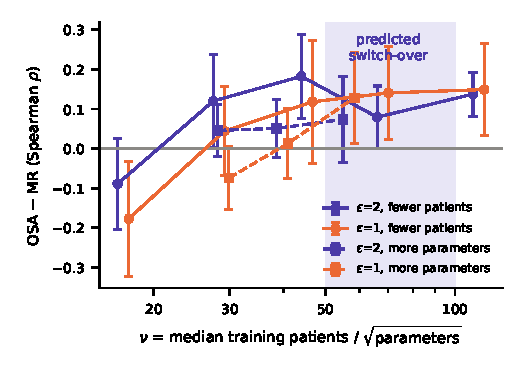
\includegraphics[width=\columnwidth]{figures/figure20_nu_sweep.pdf}
\caption{Pre-registered test: OSA$-$MR (paired difference in Spearman $\rho$ with the exact reference, 95\% CI, 20 splits) as $\nu$ is lowered within the ten largest PCa-19 hospitals, by removing patients (solid) or adding uninformative parameters (dashed). Shaded: the switch-over predicted before the test. Points at the same $\nu$ are offset slightly for legibility.}
\label{fig:nu}
\end{figure}

\subsection{The Revised Rule}
\begin{enumerate}
    \item \emph{Count the cost.} Report the composed $\varepsilon$ of any valuation (Proposition~2) and do not retrain coalitions at a per-run budget; retraining was not accurate in any setting.
    \item \emph{Without DP on the releases} (for example, when model sharing is covered by a data-use agreement), use OSA-Shapley, the most accurate valuation in all four settings ($\rho$ \mlpOsaNoDP--\osaNoDP).
    \item \emph{Under DP with a convex model}, OSA-Shapley is at least as accurate as MR down to $\nu\approx30$ at $\varepsilon=2$ and $\nu\approx40$ at $\varepsilon=1$; below that, use MR, which adds no privacy cost when the federation already trains with DP-FedAvg.
    \item \emph{With a non-convex model}, use MR.
    \item \emph{Check hospital size before using it.} Size matched contribution only where hospitals differed mainly in volume (\pxSSizeTwo{} for the ten smallest PCa-19 hospitals) and failed elsewhere (\pxLSizeTwo{} and \hrSizeTwo). Neither size nor summary statistics can detect bad data; the score of a single released model can.
    \item \emph{Compute both OSA-Shapley and MR when in doubt.} $\nu$ does not explain every case: the heart-disease federation ($\nu=\nuHeart$) favoured MR although the sweep says OSA should be competitive there. Its four hospitals make $\rho$ coarse, and site-specific missing data make some features constant within a hospital, so single-hospital models are poorly determined; both explanations are untested. Disagreement between the two valuations is a sign that the ranking is not resolved at the chosen budget, and with small $\nu$ at $\varepsilon\le1$ coarse credit (equal shares plus screening for bad data) is the honest fallback.
\end{enumerate}
